\documentclass[12pt]{book}
\usepackage{graphicx}
\usepackage{amsmath,amssymb,fullpage,cancel,hyperref}
\usepackage{tikz,tcolorbox}
\usepackage[miktex]{gnuplottex}
\usepackage{titlesec}
\usepackage[Bjornstrup]{fncychap}
\usepackage{lscape}
\usepackage{import}
\usepackage{breqn}
\tcbuselibrary{theorems}
\newcommand{\ds}{\displaystyle}
\allowdisplaybreaks
\setcounter{tocdepth}{4}
\setcounter{secnumdepth}{4}
\usepackage[titles]{tocloft}
\makeatletter
\newcommand*{\tocwithouttitle}{\@starttoc{toc}}
\makeatother
\usepackage{pgfplots, pgfplotstable}
\pgfplotsset{compat=1.8}

\renewcommand{\labelitemii}{$\diamond$}

\newcommand{\sep}{\vskip .7in}
\newcommand{\ansbox}[1]{%
\hbox to 1.5 truein{\hfil \framebox{\parbox[b]{#1in}{\quad \\ \quad}}}}
%%%%%%%%%%%%%%%%%%%%%%%%%%%%%%%%%%%%%%%%%%%%%%%%%%%%%%%%%%%%%%%%%%%%%%%%%
\baselineskip =20pt
\parskip =10pt
\newcommand{\ts}{\textsuperscript}
\newtheorem{theorem}{Theorem}
\newtheorem{alg}{Algorithm}
\newtheorem{case}{Case}
\newtheorem{scase}{Case}[case]
\newtheorem{sscase}{Case}[scase]
\newtheorem{ssscase}{Case}[sscase]
\newtheorem{sssscase}{Case}[ssscase]
\newtheorem{claim}{Claim}
\newtheorem{prop}{Proposition}
\newtheorem{cor}{Corollary}
\newtheorem{defn}{Definition}
\newtheorem{lemma}{Lemma}
\newtheorem{note}{Note}
\newtheorem{fact}{Fact}
\newtheorem{game}{Game}
\newtheorem{strat}{Strategy}
\newtheorem{ex}{Example}
\newtheorem{prob}{Problem}
\newtheorem{rul}{Rule}
\newtheorem{remark}{Remark}
\newtheorem{objec}{Objective}
\newtheorem{hwk}{Homework}
\newtheorem{step}{Step}
\newtheorem{rvw}{Review}

%**********Highlighted Theorems and Defs**********
\newtcbtheorem{imp:thm}{Theorem}%
{colback=blue!5,colframe=blue!35!black,fonttitle=\bfseries}{th}
\newtcbtheorem{imp:defn}{Definition}%
{colback=blue!5,colframe=blue!35!black,fonttitle=\bfseries}{th}
\newtcbtheorem{imp:rule}{Rule}%
{colback=blue!5,colframe=blue!35!black,fonttitle=\bfseries}{th}
\newtcbtheorem{imp:form}{Formula}%
{colback=blue!5,colframe=blue!35!black,fonttitle=\bfseries}{th}
\newtcbtheorem{imp:ex}{Example}%
{colback=blue!5,colframe=blue!35!black,fonttitle=\bfseries}{th}
%*************************************************

\newenvironment{sol}%
{%
\noindent{\it Solution.}
}%
{%
 \quad\hfill$\blacktriangledown$\vspace*{2ex}
}

%***Graphing Code
%\begin{tikzpicture}[domain=-2:3,xscale=.6,yscale=.6]
%\draw[thin,color=gray!40] (-2.1,-2.1) grid (3.1,8.1);
%\draw[->,thick] (-2.2,0) -- (3.2,0) node[right] {x};
%\draw[->,thick] (0,-2.2) -- (0,8.2) node[above] {y};
%\draw[thick,color=blue,domain=-2:3,samples=200] plot[id=ex1a] function{(x-1)**2-1} node[right] {$f$};
%\end{tikzpicture}

\title{MAT 330 - Differential Equations}
\author{Mr. Ryan Evaul\\
Southern New Hampshire University}

\begin{document}
%\frontmatter
\maketitle
%\tableofcontents

\chapter*{\contentsname}
\markboth{\MakeUppercase{\contentsname}}{\MakeUppercase{\contentsname}}
\tocwithouttitle
%\begin{landscape}
% !TEX root = /Users/us2009801/Documents/GitHub/DifferentialEquations/main.tex
\chapter{Class 1 - Thursday, January 19\ts{th}, 2017}
\section{\S 1 Differential Equations}

\begin{remark} $\dfrac{dx}{dt}=f'(x,t) \implies $rate of change of $x$ (state variable) with respect to time.
\begin{itemize}
\item Newton:$$y'=ky,y>0$$
\item Leibniz:$$\dfrac{dx}{dt}=kx,x>0$$

\begin{align*}
    k<0 & \implies \text{decay}\\
    k>0 & \implies \text{growth}\\
    \dfrac{dx}{dt} & =kx\\
    dx & =(kx)dt\\
    \frac{1}{x} dx & = k dt\\
    \textcolor{red}{\int} \frac{1}{x} dx & =\textcolor{red}{\int} k dt\\
    ln|x| & = kt+c\\
    \textcolor{red}{e}^{\textcolor{red}{(}ln|x|\textcolor{red}{)}} & = \textcolor{red}{e}^{\textcolor{red}{(}kt+c\textcolor{red}{)}}\\
    x & = e^{kt+c} = e^{c}e^{kt}\\
    x & = Ae^{kt} \leftarrow \text{A is a constant}
\end{align*}
\item verify:
\begin{align*}
    x & =Ae^{kt}\\
    \dfrac{dx}{dt} & =kAe^{kt} \leftarrow Ae^{kt} = x\\
    & = kx
\end{align*}
Also $x=0$ is a solution if there are no restrictions on x
$$\textcolor{red}{\dfrac{dx}{dt} = 0 = k*0 = kx}$$
\end{itemize}
\end{remark}
\section{\S 2 Definitions}
\begin{align*}
    \text{Set} & : \text{Collection of Objects}\\
    \text{Element} & : \text{Member of Set}\\\\
    \text{Domain of }f & : \text{Set of all independent value inputs of} f\\
    \text{Range of }f & : \text{Set of Dependent Values}\\
    f & : 0 \rightarrow \mathbb{R}, f(x)=y
\end{align*}
\begin{remark} Function of 2 independent variables:\\
If $(x,y)\in \epsilon$ maps to unique $z$, then $z=f(x,y)$ 
\end{remark}
\begin{remark} Region$\rightarrow \epsilon$: Set in plane if:\\
\begin{enumerate}
  \item Each point $p \in \epsilon$, $p$ is the center of a circle whose interior is also in $\epsilon$
  \item Every two points in $\epsilon$ can be connected by a curve entirely in $\epsilon$
\end{enumerate}
\end{remark}
\begin{imp:defn}{Implicit Function}{} Relation $f(x,y)=0$ defines $y$ as an implicit function of $x$ on $I:a<x<b$ if there exists $g(x)$ defined on $I$ such that $f[x,g(x)]=0$, $\forall x \in I$.
\end{imp:defn}
\begin{remark} $f(x,y)=16-x^{2}-y^{2}$ relation
Looking for $g(x)$ such that
\begin{align*}
    0 & = (16-x^{2})-[g(x)]^{2}\\
    g(x) & = \sqrt{16-x^{2}}\\
    0 & = 16-x^{2}-(16-x^{2})\\
    0 & = 16-x^2-16+x^{2}\\
    g(x) & = -\sqrt{16-x^{2}}
\end{align*}
\end{remark}
\begin{remark}Elementary Functions $\rightarrow$ Building Blocks to Work With
\begin{enumerate}
    \item Power Functions: $x^{n}$
    \item Root Functions: $x^{\frac{1}{n}}$
    \item Exponential Functions: $e^{x}$
    \item Log Functions: $log(x)$
    \item Trig Functions:
    \item Inverse Trig:
\end{enumerate}
\end{remark}
\section{\S 3 Differential Equations}
\begin{imp:defn}{Ordinary Differential Equation (ODE)}{} Let $f(x)$ define a function of $x$ on $I$:$a<x<b$ Then an ordinary differential equation (ODE) involves $x$, $f(x)$, and one or more derivatives of $f$
\end{imp:defn}
\begin{note} $I$ is our typical interval, & lazy, so won't write $a<x<b$.
\end{note}
\begin{remark}Order of Ordinary Differential Equation is order of the highest derivative
\begin{align*}
    f^{(4)}(x)+2f^{(2)}(x)+x & =0\\
    f''''(x)+2f''(x)+x & = 0
\end{align*}
\end{remark}
\begin{remark}Solution $x$ satisfies an ODE if when you substitute $x$ into ODE, it is a true statement.
\end{remark}
\begin{ex}
\begin{align*}
    y' & =e^{x}\\
    y & =e^{x}
\end{align*}
\end{ex}
\begin{ex}Differential Equation:
\begin{align*}
    (1+x^{2})y' & =xy\\
    y & = \sqrt{1+x^{2}}
\end{align*}
\end{ex}
% !TEX root = /Users/us2009801/Documents/GitHub/DifferentialEquations/main.tex
\chapter{Class 2 - Monday, January 23\ts{rd}, 2017}
\section{\S 3 Ordinary Differential Equations}
\begin{imp:defn}{Ordinary Differential Equation}{} Let $f(x)$ be a function of $x$ on interval $I$ then ODE involves $x,f(x)$ \& 1 or more derivatives of $f$. Order of an ODE is highest derivative of $f$.\\
Recall: $y=f(x)$ is solution of an ODE if when you plug in $y, y', y''...$ as necessary, equation holds.
\end{imp:defn}
\begin{imp:defn}{Explicit Definition of Solution}{} Let $y=f(x)$, define $y$ as a function of $x$ on $I$. $f(x)$ is an explicit solution (or simply a solution) if for all $x\in I$, $F(x, f(x), f'(x),...f^{(n)})=0$
\end{imp:defn}
\begin{ex}
\begin{align*}
    e^{x-y}+(e^{y-x})\dfrac{dy}{dx} & =0\\
    e^{2y}+e^{2x} & =1\\
    F(x, f(x), f'(x)=0 \rightarrow [(e^{x-f(x)})+(e^{f(x)-x})(f'(x)) & = 0]
\end{align*}
\begin{align*}
    \text{Look at: }e^{2y}+e^{2x} & = 1\\
    2\,\dfrac{dy}{dx}\, e^{2y}+2e^{2x} & = 0\\
    \dfrac{dy}{dx} & = \frac{-e^{2x}}{e^{2y}} = -e^{2x-2y}
\end{align*}
Now plug it into the ODE $$e^{x-y}+(e^{y-x})(-e^{2x-2y})=e^{x-y}-e^{x-y}=0$$
\end{ex}
\section{\S 4 General Solution of ODEs}
\begin{imp:defn}{Parameter}{} Let $y=f(\textcolor{red}{x}; \textcolor{blue}{c_1}, \textcolor{blue}{c_2}) = 2x+3+ c_1e^x+c_2e^{2x}$\\
   $ \textcolor{red}{x} \& \leftarrow \text{variable}$\\
    $\textcolor{blue}{c} \& \leftarrow \text{Parameters - Constants that vary with initial conditions}$
\end{imp:defn}
\begin{ex} Given an equation with parameters, how do you show it is or isn't a solution for an ODE? \textcolor{red}{Plug in, check if equals zero.}
\end{ex}
\begin{ex}
Given a solution, how do you determine an ODE for which the Solution satisfies?\\
\begin{align*}
    x^2-cy+c^2 &=0 \leftarrow c=\text{constant}\\
    2x-cy' &=0\\
    y' &= \frac{1}{c}*2x \leftarrow \text{if} c\neq 0\\
    \textcolor{red}{\text{Let's Square }} y'&=\frac{1}{c}*2x\\
    (y')^2&=\frac{4}{c^2}x^2\\
    \textcolor{red}{\text{Multiply Both Sides by }(y')^2 \rightarrow} (x^2-cy+c^2)(y')^2&=0\textcolor{red}{(y')^2}=0\\
    x^2(y')^2-cy(\frac{4}{c^2}x^2)+4x^2&=0\\
    \textcolor{red}{\text{Note: }\frac{4}{c}yx^2=2xy(\frac{2}{c}x)}&=\textcolor{red}{2xy(y')}\\
    \rightarrow x^2(y')^2-2xy*y'+4x^2&=0 \leftarrow \text{ is the ODE!}
\end{align*}
\end{ex}
\section{\S 4C Initial Conditions}
\begin{imp:defn}{Particular Solution}{} A particular solution of a differential equation satisfies the differential equation but also has no arbitrary constants.
\end{imp:defn}
\begin{note}
If we have $n$ parameters in a solution, we need $n$ initial conditions
\end{note}
\begin{ex}
Initial Condition $\rightarrow$ $y \left( 3 \right) =1$\\
\begin{align*}
    \dfrac{dy}{dx} & = y \\
    \text{ODE} \rightarrow y'-y & = 0\\
    \dfrac{dy}{dx} & =y\\
    1dy&= ydx\\
    \int \frac{1}{y}dy &=\int dx \text{ if } y\neq 0\\
    \ln \left| y \right| +c &=x+c\\
    \ln \left| y \right| &=x+c_1\\
    y &=e^{x+c_1}\\
    y &=e^{c_1}e^x=Ae^x\\
    \text{Use Initial Condition} \rightarrow 1&=Ac^3\\
    A &=e^{-3}\\
    y &= e^{x-3}
\end{align*}
\end{ex}
\section{\S Direction Fields}
\begin{note}
There should be a graph here.
\end{note}
Given $y=f(x)$ or $f(x,y)=0$ on $I$ and $y'$ is defined as $\dfrac{dy}{dx}=f'(x)$. Then $y'$ gives the slope of the graph of $f(x)$ at each point $x \in I$.
\begin{imp:defn}{Integral Curve}{} If $y=f(x)$ satisfies $y'=F(x,y)$ then graph of $f(x)$ called the integral curve.
\end{imp:defn}
\begin{ex}
How to draw direction field:
\begin{center}
 \begin{tabular}{|c||c|c|c|c|} 
 \hline
 \multicolumn{5}{|c|}{$y'=2x+y$} \\
 \hline
 x\backslash y & -1 & 0 & 1 & 2\\
 \hline\hline
 -1 & \textcolor{red}{-3} &  &  &  \\ 
 \hline
 0 &  &  &  &  \\
 \hline
 1 &  &  &  &  \\
 \hline
 2 &  &  &  &  \\
 \hline
\end{tabular}
\end{center}
Entries are $y'$ evaluated at $(x,y)$ point. \textcolor{red}{$y'(-1,-1)=2(-1)+(-1)=-3$}


 \begin{figure}[h!]

    \begin{subfigure}{\textwidth}
    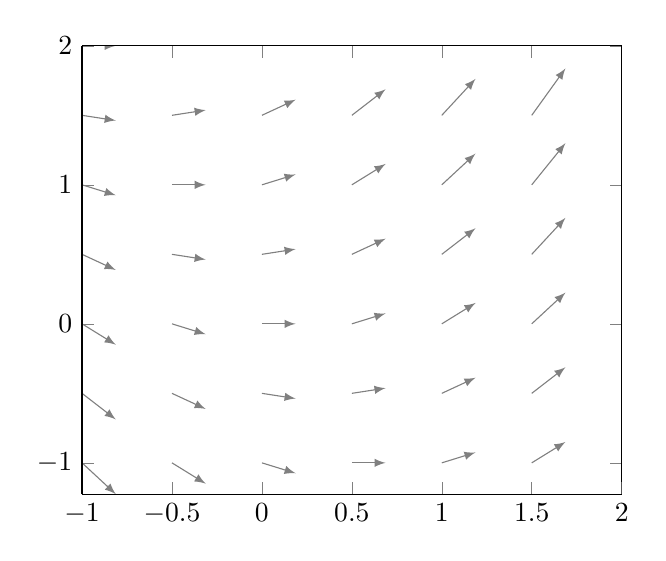
\begin{tikzpicture}

    \begin{axis}[
        view={0}{90},
        domain=-1:2,
        y domain=-1:2,
        xmax=2, ymax=2,
        samples=7
    ]
    \addplot3 [gray, quiver={u={2.5}, v={2*x+y}, scale arrows=0.075,
every arrow/.append style={-latex}}] (x,y,0);
    %\addplot [thick, red] table [x=x, y=y] {\loadedtable};
    \end{axis}
    \end{tikzpicture}
    
    \end{subfigure}

\end{figure}
\end{ex}
% !TEX root = /Users/us2009801/Documents/GitHub/DifferentialEquations/main.tex
\chapter{Class 3 - Thursday, January 26\ts{th}, 2017}
\begin{hwk}
The following item appeared in a newspaper. "The expedition used the carbon-14 test to measure the amount of radioactivity still present in the organic material found in the ruins, thereby determining that a town existed there as long ago as 7000 B.C." Using the half-life figure of $C^{14}$ as given in the text, determine the approximate percentage of $c^{14}$ still present in the organic material at the time of the discovery.\\\\
Half Life = 5,600 years (After 5,600 years, 50\% is gone). Therefore determine the percent present at discovery.\\
\begin{center}
\begin{tabular}{|c|c|c|c|c|}
\hline
\multicolumn{2}{|c|}{At 7,000 B.C.} &  & \multicolumn{2}{|c|}{At 1,940 A.D.}\\
\hline
$t=0$ & $y=1$ &  & $t=8940$ & $\%=$? \\
\hline
\end{tabular}
\end{center}
\begin{align*}
    \dfrac{dy}{dt}&=-ky\\
    \int \frac{1}{4} dy &= \int -k dt\\
    \ln|y|&=-kt\\
    \text{General Solution} \rightarrow y&=Ce^{-kt}\\
    1&=Ce^{-k(0)}\\
    1&=C\\
    y&=e^{-kt}\\
    .5&=e^{-5600k}\\
    \ln (.5)&=\ln(e^{-5600k})\\
    \ln(.5)&=-5600k\\
    \frac{\ln(.5)}{-5600}&=k\\
    \frac{\ln (2)}{5600}&=0.000124\\
    k&=1.24e^{-4}\\
    y&= e^{-(1.24e^{-4})(8940)}\\
    y&=.325\\
    y&=32.5\% \text{ Remaining}
\end{align*}
\end{hwk}

\section*{\S 6 Separable Differential Equations}
\begin{align*}
    f'(x)&=\dfrac{dy}{dx}\\
    dy&=f'(x)dx\\
    &=f'(x)\Delta x \text{ for small } \Delta\\
    \textcolor{red}{\text{Notation} (\star )} \rightarrow \textcolor{red}{P(x,y)dx+Q(x,y)dy}&=\textcolor{red}{0}\\
    P(x,y)+Q(x,y) \dfrac{dy}{dx}&=0
\end{align*}
\begin{imp:defn}{Separable Differential Equation}{} An ODE is separable if $(\star )$ can be written as:
\begin{align*}
  f(x)dx+g(y)dy&=0 \\
  \rightarrow \int f(x)dx+\int g(x)dy &=c
\end{align*}
\end{imp:defn}
\begin{ex}
\begin{align*}
    xdy-ydx&=0\\
    xdy&=ydx \leftarrow \text{ if } x,y\neq 0\\
    \int \dfrac{1}{y} dy &= \int \dfrac{1}{x} dx\\
    \ln |y|+c_1 &= \ln |x| +c_2\\
    e^{\ln |y|} &= e^{\ln |x|} +c\\
    y &= cx
\end{align*}
\end{ex}
\begin{ex}
\begin{align*}
    (x-1)cos(y) dy &= (2x)sin(y) dx\\
    \frac{(x-1)cos(y)}{sin(y)} dy &= \frac{(2x)sin(y) dx}{sin(y)}\\
    \frac{(x-1)cos(y)}{sin(y)} dy &= (2x)dx\\
    \frac{(x-1)cos(y)}{sin(y)(x-1)} dy &= \frac{(2x)}{(x-1)}dx\\
    \frac{cos(y)}{sin(y)} dy &= \frac{(2x)}{(x-1)}dx\\
    \int \frac{cos(y)}{sin(y)} dy &= \int \frac{(2x)}{(x-1)}dx\\
    \textcolor{blue}{u} &= \textcolor{blue}{sin(y)}\\
    \textcolor{blue}{du} &= \textcolor{blue}{cos(y)dy}\\
    \ln |sin(y)| &= \int \frac{(2x)}{(x-1)}dx\\
    \ln |sin(y)| &= 2\int \frac{(x)}{(x-1)}dx  \textcolor{red}{ +\frac{-1+1}{1}=0 \leftarrow \text{ Fancy 1}}\\
    \ln |sin(y)| &= 2\int \frac{(x-1)+1}{(x-1)}dx\\
    \ln |sin(y)| &= 2\int 1+ \frac{1}{(x-1)}dx\\
    \ln |sin(y)| &= 2 \left[ x +\ln \left| x-1 \right| \right]+c\\
    \ln |sin(y)| &= 2x +2 \ln \left| x-1 \right| +c\\
    e^{\ln |sin(y)|} &= e^{2x +2 \ln \left| x-1 \right| +c}\\
    sin(y) &= e^{2x +2 \ln \left| x-1 \right| +c}\\
    sin(y) &= (x-1)^2*e^{2x+c}\\
\end{align*}
\end{ex}
\section*{\S 7}
\begin{ex}
\begin{align*}
    (x^2+y^2)dx &= 2xydy\\
    \frac{x^2 dx}{x}+\frac{y^2 dx}{x}&=\frac{2xy dy}{x}\\
    xdx+\frac{y^2}{x}dx&=2ydy\\
    \frac{xdx+\frac{y^2}{x}dx}{\textcolor{red}{y^2}}&=\frac{2ydy}{\textcolor{red}{y^2}}\\
    \frac{x}{y^2} dx+ \frac{1}{x}dx &= \frac{2}{y}dy\\
    \left( \frac{x^2}{y^2} +1 \right) dx &= \frac{2xy}{y^2}dy\\
    \left( \left[ \frac{x}{y} \right]^2 +1 \right) dx &= 2 \left[ \frac{y}{x} \right] dy\\
    \left[  1+ \left( \frac{y}{x}\right) ^2  \right] dx &= 2 \left[ \frac{y}{x} \right] dy\\
    \textcolor{blue}{u} &= \textcolor{blue}{\frac{y}{x}}\\
    \textcolor{blue}{y} &= \textcolor{blue}{ux}\\
    \textcolor{blue}{dy} &= \textcolor{blue}{udx+xdu}\\
    \left( 1+u^2 \right)dx &= 2u \left( udx+xdu \right)\\
    1dx+u^2dx &= 2u^2dx+2xudu\\
    1dx+-u^2dx &= 2xudu\\
    \left( 1-u^2 \right) dx &= 2x u du\\
    \textcolor{blue}{\frac{1}{x}} * \frac{\left( 1-u^2 \right) }{\textcolor{red}{1-u^2}} dx &= \frac{2x}{\textcolor{blue}{x}} * \frac{u du}{\textcolor{red}{1-u^2}}\\
    \frac{1}{x}dx &= 2\frac{u}{1-u^2}du\\
    \int \frac{1}{x}dx &= \int 2\frac{u}{1-u^2}du\\
    \ln |x| &= \ln |1-u^2|^{-1}+c\\
    x &= \frac{1}{1-u^2}*e^c\\
    1-u^2 &= \frac{1}{x} *c\\
    1-\left[ \frac{y}{x} \right] ^2 &= \frac{1}{x}*c\\
    \textcolor{red}{y(-1)} &= \textcolor{red}{0}\\
    1-\left[ \frac{0}{-1} \right]^2 &= \frac{1}{-1}*c\\
    \textcolor{red}{c} &= \textcolor{red}{-1}\\
    1-\frac{y^2}{x^2} &= - \frac{1}{x}\\
    y^2 &= x^2+x\\
\end{align*}
\end{ex}
\begin{imp:defn}{Homogeneous Function}{} The Equation $z=f(x,y)$ is Homogeneous of order n if $f(x,y)=x^n*g(u)$ for %u=\frac{y}{x}$
\end{imp:defn}
\begin{imp:defn}{1\ts{st} Order Ordinary Differential Equation with Homogeneous Coefficients}{} Let $$(\star ) \rightarrow P(x,y) dx+Q(x,y)dy=0$$ where $P(x,y)$ and $Q(x,y)$ are homogeneous functions of order n.
\end{imp:defn}
\begin{imp:thm}{} IIf coefficients in $(\star )$ are each homogeneous functions of order n, then $y=ux$ and $dy=udx+xdu$ leads to a separable equation.\\
Verify the Coefficients in the example are homogeneous:\\
\begin{align*}
    \left( x^2+y^2\right) dx &= 2xy*dy\\
    0 = P(x,y) &= x^2 + y^2\\
    1+\frac{y^2}{x^2} &= g(u)\\
    u&= \frac{y}{x} \leftarrow \textcolor{red}{\text{0\ts{th} order}}\\
    g(u) &= 1+u^2\\
    Q(x,y) &= -2xy\\
    0 &= -2xy\\
    0 &= -\frac{2y}{x}\\
    -2u &= g(u) \leftarrow \textcolor{red}{\text{0\ts{th} order}}
\end{align*}
\end{imp:thm}
% !TEX root = /Users/us2009801/Documents/GitHub/DifferentialEquations/main.tex
\chapter{Class 4 - Monday, January 30\ts{th}, 2017}
\begin{hwk}
\S6 $\#$9\\
\begin{align*}
    e^{x+1}\tan y \,dx+\cos y \,dy&=0\\
    e^{x+1}dx &= -\frac{\cos y}{\tan y}dy\\
    \int e^{x+1} \,dx &= \int - \frac{\cos^2 y}{\sin y} \,dy\\
    e^{x+1} \,dx &= \int - \frac{1-\sin^2 y)}{\sin y} \,dy\\
    \text{Note: }1 &= \textcolor{red}{\cos^2 y+\sin^2 y}\\
    e^{x+1}&=- \int\frac{1}{\sin y} - \sin y \,dy\\
\end{align*}
\end{hwk}
\begin{hwk}
\S7 $\#$7\\
\begin{align*}
    y^2 \,dx +\left[x \sqrt{y^2-x^2}-xy \right] \,dy &=0\\
    y^2 \,dx +\left[x \sqrt{x^2\left( \frac{y^2}{x^2}-1\right) }-xy \right] \,dy &=0\\
    y^2 \,dx +\left[x*x \sqrt{\frac{y^2}{x^2}-1}-xy \right] \,dy &=0\\
   y^2 \,dx +\left[x^2 \sqrt{\frac{y^2}{x^2}-1}-xy \right] \,dy &=0\\
  \frac{y^2}{x^2} \,dx +\left[\frac{x^2 \sqrt{\frac{y^2}{x^2}-1}}{x^2}-\frac{xy}{x^2} \right] \,dy &=0\\
  \frac{y^2}{x^2} \,dx +\left[\sqrt{\frac{y^2}{x^2}-1}-\frac{y}{x} \right] \,dy &=0\\
  u&= \frac{y}{x}\\
  y&= ux\\
  dy&= u\,dx+x\,du\\
  u^2 \,dx +\left[ \sqrt{u^2-1} -u \right] *\left[ u\,dx +x\,du \right] &=0\\
  u^2 \,dx +\left[ \sqrt{u^2-1} -u \right] *u\,dx + \left[ \sqrt{u^2-1} -u \right] x\,du &=0\\
  \left[ u^2+u\sqrt{u^2-1}-u^2\right]\,dx + \left[\sqrt{u^2-1}\right]x\,du &=0\\
  \left[u\sqrt{u^2-1}\right]\,dx + \left[\sqrt{u^2-1}\right]x\,du &=0\\
  \frac{\left[u\sqrt{u^2-1}\right]}{\left[u\sqrt{u^2-1}\right]}\,dx &= -\frac{\left[\sqrt{u^2-1}\right]}{\left[u\sqrt{u^2-1}\right]}x\,du\\
  \frac{1}{x}\,dx &= -\frac{\left[\sqrt{u^2-1}\right]}{\left[u\sqrt{u^2-1}\right]}\frac{x}{x}\,du\\
  \frac{1}{x}\,dx &= -\left[ \frac{1}{u} - \frac{1}{\sqrt{u^2-1}} \right] \,du
\end{align*}
\end{hwk}
\section*{\S 8C Linear Coefficient, Non-Homogeneous, Non-Parallel}
$(\star ) \rightarrow P(x,y)dx +Q(x,y)dy=0$\\
If $P(x,y)= a_1x+b_1y+c_1$ and $Q(x,y)= a_2x+b_2y+c_2$ are both linear functions and where $c_1, c_2$ are both not zero.\\
If $\frac{a_1}{b_1}\neq \frac{a_2}{b_2}$ then the slope of the the lines are not equal and $\exists !$ (there exists unique) point of intersection.\\
Let:
\begin{align*}
    u=P(x,y)&=a_1x+b_1y+c_1\\
    v= Q(x,y)&= a_2x+b_2y+c_2\\
    du&= a_1dx+b_1dy\\
    dv&=a_2dx+b_2dy
\end{align*}
Then if we solve for $dx$, $dy$ and substitute in, this gives ordinary differential equation with homogeneous coefficients $\rightarrow$ \S 7.
\begin{ex}
\begin{step} Find u, v, du, dv
\begin{align*}
    (x=2y)dx+(y-1)dy&=0\\
    u&= x+2y\\
    du&= dx+2dy\\
    y&= y-1\\
    dy&= dy\\
    \end{align*}
\end{step}
\begin{step} Solve for dx,dy in terms of du,dv
    \begin{align*}
    dx&= du-2dy\\
    dy&=dv\\
    dx&= du-2dv
    \end{align*}
\end{step}
\begin{step} Sub into Original Equation
    \begin{align*}
    u(du-2\,dv)+,v\,dv&=0\\
    u\,du-s\,dv+v\,dv&=0
    \end{align*}
\end{step}
\begin{step} Check for Homogeneity $\rightarrow$ can write $Q(x,y)$ as $x^n*g\left(\frac{y}{x}\right)$
    \begin{align*}
    \textcolor{red}{\text{Yes, Homogeneous Coefficients}} \rightarrow \frac{u}{v}du+\left( -\frac{2u}{v}+1\right) dv &=0 \\
    u\,du+(-2u+v)dv&=0
    \end{align*}
\end{step}
\begin{step} Sub into Original Equation
    \begin{align*}
    y&=ux\\
    u&=tv\\
    du&= t\,dv+v\,dt\\
    tv(t\,dv+v\.dt)+(-2tv+v)dv&=0\\
    \text{Algebra}\\
    tv^2\,dt + (^2-2t+1)v\,dv&=0
    \end{align*}
\end{step}
\begin{step} Separate, Use \S 6 Techniques
    \begin{align*}
    \frac{t}{t^2-2t+1}dt+\frac{1}{v}dv &= 0\\
    t&\neq -1\\
    v&\neq 0\\
    \int \frac{t \textcolor{red}{-1+1}}{(t-1)^2}dt&= \int \frac{t-1}{(t-1)^2}+\frac{1}{(t-1)^2}\,dt\\
    \int \frac{1}{t-1}dt&= \int \frac{1}{(t-1)}+(t-1)^{-2}\,dt\\
    \int \frac{1}{t-1}dt&=\ln|t-1|+-(t-1)^{-1}\\
    \ln |t-1|-(t-1)^{-1} + \ln|v|&=c
    \end{align*}
\end{step}
\begin{step} Back Substitute
    \begin{align*}
    t&=\frac{u}{v}\\
    u&= x+2y\\
    v&= y-1\\
    \ln \left| \frac{x+2y}{y-1} -1 \right| - \left(\frac{x+2y}{y-1} -1 \right) ^{-1} +\ln |y-1|&=c
\end{align*}
\end{step}
\end{ex}
\section*{\S 8D Parallel Lines}
\begin{ex}
\begin{align*}
    (3x+2y+1)dx+(3x+2y-1)dy&= 0\\
    u&= 3x+2y+1\\
    du&= 3dx+2dy\\
    dy&= \frac{du-3dx}{2}\\
    u\,dx+(u-2) \left(\frac{1}{2}du-\frac{3}{2}dx \right) &=0\\
    u\,dx + \frac{1}{2}u\,du - du-\frac{3}{2}u\,dx+3dx&=0\\
    \left( -\frac{1}{2}u +3 \right) dx + \left(\frac{1}{2}u-1 \right)du&= 0\\
    dx&= \frac{1-\frac{1}{2}u}{-\frac{1}{2}u+3}du\\
    dx&=\frac{2-u}{-u+\frac{3}{2}}du\\
    \int dx&= \int \frac{2-u}{-u+\frac{3}{2}}du\\
    \int dx&= \int \frac{2-\frac{3}{2}+\left( -u+\frac{3}{2}\right)}{\frac{3}{2}-u}du\\
    \int dx&=\int \frac{1}{2}* \frac{1}{\frac{3}{2}-u}+1 du\\
    \int dx&= \int \frac{1}{3-\frac{u}{2}}+1\,du\\
    v&= 3-\frac{u}{2}\\
    dv&=-\frac{1}{2}du\\
    -2dv&=du\\
    x&= -2\ln \left| 3-\frac{u}{2}\right| +u +c\\
    x&= -2\ln\left| 3-\frac{1}{2}(3x+2y+1) \right| +3x+2y+1+c\\
    c&= \text{...}
\end{align*}
\end{ex}
\chapter{Class 5 - Thursday, February 2\ts{nd}, 2017}
\section*{\S 8.1}
\begin{ex} Let:
\begin{align*}
    (x+2y+-4)dx-(2x-4y)dy&=0\\
    (x+2y+-4)dx+(-2x+4y)dy&=0\\
    \textcolor{red}{P(x,y)dx+Q(x,y)dy}&=0
\end{align*}
\begin{itemize}
  \item Not Separable
  \item Not Homogeneous Because $-\frac{4}{x}$ exists if we divide by $x$.
  \item Linear Coefficients
  \begin{itemize}
    \item Use \S 8 Tools
  \end{itemize}
  \item Not Parallel Lines
  \begin{itemize}
  \item  $u=P(x,y)$ and $v=Q(x,y)$
  \end{itemize}
\end{itemize}
\begin{note}
Goal: Rewrite the Equation with $u$ and $v$ such that it becomes a homogeneous equation. $\rightarrow$ use \S 7 Tools
\end{note}
\begin{center}
 \begin{tabular}{|c|c|} 
 \hline
 $u=x+2y-4$ & $v=-2x+4y$\\
 \hline
 $du=dx+2y\,dy$ & $dv=-2dx+4dy$\\ 
 \hline
\end{tabular}
\end{center}
\begin{align*}
    dx&= du-2dy\\
    dx&=du-\frac{1}{4}dv-\frac{1}{2}du\\
    dx&=\frac{1}{2}du-\frac{1}{4}du\\
    dv&=-2(du-2dy)+4dy\\
    dv&= -2du+8dy\\
    \frac{dv+2du}{8}&= dy\\
    dy&=\frac{1}{4}du+\frac{1}{8}dv
\end{align*}
\end{ex}
\begin{ex}
    $$u \left( \frac{1}{2}du-\frac{1}{4}dv \right) +v \left( \frac{1}{4}du+\frac{1}{8} dv \right) &=0$$
\begin{note}
\textcolor{red}{Trick: Multiply by 8 to clear functions.}
\end{note}
\begin{align*}
    4u\,du-2u\,dv+2v\,du+v\,dv&=0\\
    (4u+2v)du+(-2u+v)dv&=0
\end{align*}
\begin{note}
\textcolor{red}{Homogeneous since we find $\frac{v}{u}$}
\end{note}
$$\left( 4+\frac{2v}{u} \right) du+ \left( -2+\frac{v}{u} \right) dv &=0$$\\
\textcolor{red}{Let $w=\frac{v}{u}$ $\rightarrow$ $v=uw$ $\rightarrow$ $dv=u\,dw+w\,du$}
\end{ex}
\begin{ex}
    \begin{align*}
        (4+2w)du+(-2+w)(u\,dw+w\,du)&=0\\
        4du+2w\,du-2u\,dw -2w\,du+uw\,dw+w^2\,du&=0\\
        \left( 4+2w-2w+w^2 \right)du+(-2u+uw)dw&=0\\
        \left( 4+w^2 \right)du+(-2u+uw)dw&=0\\
        \left( 4+w^2 \right) du +u(-2+w)dw&=0\\
        \frac{1}{u}du + \frac{(-2+w)}{(4+w^2)}dw&=0\\
        \ln |u| - \tan^{-1} \left( \frac{w}{2} \right)+\frac{1}{2} \ln \left| 4+w^2 \right|&=c\\
        \textcolor{red}{u}&=\textcolor{red}{x+2y-4}\\
        \textcolor{red}{w}&=\textcolor{red}{\frac{-2x+4y}{x+2y-4}}\\
    \end{align*}
\end{ex}
\section*{\S 9 Exact Equations}
% !TEX root = /Users/us2009801/Documents/GitHub/DifferentialEquations/main.tex
\chapter{Class 6 - Monday, February 6\ts{th}, 2017}
% !TEX root = /Users/us2009801/Documents/GitHub/DifferentialEquations/main.tex
\chapter{Class 7 - Thursday, February 16\ts{th}, 2017}

\chapter{Class 8 - Monday, February 20\ts{th}, 2017}
% !TEX root = /Users/us2009801/Documents/GitHub/DifferentialEquations/main.tex
\chapter{Class 9 - Thursday, February 23\ts{rd}, 2017}
% !TEX root = /Users/us2009801/Documents/GitHub/DifferentialEquations/main.tex
\chapter{Class 10 - Monday, February 27\ts{th}, 2017}
\section*{\S 21 Non-Homogeneous Equation with Constant Coefficients}
\begin{align*}
    \star a_n y^n+a_{n-1}y{n-1}+\text{...}+a_1y'+a_0 y&=Q(x)\\
    &\neq 0 \leftarrow \text{Non-Homogeneous}\\
    y(x)&=y_c(x)+y_p(x)\\
    y_c(x)&=\text{Solution to Homogeneous}\\
    y_p(x)&=\text{Particular solution to solve } Q(x)\\
\end{align*}
\begin{imp:defn}{Method of Undetermined Coefficients (Muc)}{} Only used when $Q(x)$ consists of sums or combinations of:$$a, x^k,e^{ax},\sin (\beta x). \cos (\beta x)$$
\end{imp:defn}
\begin{case}
No term in $Q(x)$ is similar to a term in $y_c(x)$ to the differential equation.\\
$y_p$ will be linear combination of terms presents in $Q(x)$ and all derivatives of those terms.
\begin{align*}
    y''+3y'+2y&=12e^x
    \end{align*}
\begin{step} Always find your complementary equation and build $y_c$ first
    \begin{align*}
    m^2+3m+12&0\\
    (m+2)(m+1)&=0 \rightarrow m=-1, m=-2\\
    y_c&=c_qe^{-x}+c_2e^{-2x}
    \end{align*}
\end{step}
\begin{step} Check for matching (Up to a Coefficient terms between $y_c$ and $Q(x)$
    \begin{align*}
    \text{No Matching Terms}
    \end{align*}
\end{step}
\begin{step} Find the shape of $y_p$
    \begin{align*}
    Q(X)&=12e^x\\
    y_p&=Ae^x\\
    y_p'=Ae^x\\
    y_p''=Ae^x
    \end{align*}
\end{step}
\begin{step} Take (enough) derivatives of $y_p$ so we can substitute back into the original Differential Equation
    \begin{align*}
    y_p''+3y_p'+2y_p&=12e^x\\
    Ae^x+3Ae^x+2Ae^x&=12e^x
    \end{align*}
\end{step}
\begin{step} Solve for Constants and Replace in $y_p$
    \begin{align*}
    6Ae^x&= 12e^x \rightarrow a=2, y_p=2e^x
    \end{align*}
\end{step}
\begin{step} Add $y_c$ and $y_p$ to form general solution for $y$
    \begin{align*}
    y&= c_1e^{-x}+c_2e^{-2x}+2e^x\\
    y_c&=c_1e^{-x}+c_2e^{-2x}\\
    y_p&=2e^x
\end{align*}
\end{step}
\end{case}
\begin{case}
Let $u(x)$ be a term in $y_c$. If $Q(x)$ contains a term of form $x^k+u(x), k\get 0$ then $y_p$ in linear combination of $x^{k+1} * u(x)$ and all linearly independent derivatives.
\begin{align*}
    y''+y&=\sin (x)\\
    m^2+1&=0 \rightarrow m=\pm i, \alpha =0, \beta =1\\
    y_c&= c_1 \cos (x) + c_2 \sin(x)\\
    u(x)&= \sin x \text{ then } x^\textcolor{red}{0}*\sin (x) \text{is in Q(x)}\\
    \textcolor{red}{k}&= \textcolor{red}{0}
    \end{align*}
\begin{step} $y_p$ has $x^1*\sin (x)$ and all Linear Independent Derivatives.
    \begin{align*}
    \frac{d}{dx} [q]&= x*\cos (x) +  \sin (x)\\
    q''&= -x*\sin (x)+ \cos x + \cos x\\
    q'''&= -x\cos x + - \sin x +-2 \sin x\\
    y_p&= Ax * \sin x +B x \cos x +C \sin x + D \cos x\\
    \textcolor{red}{\text{Recall }y}&=\textcolor{red}{y_c+y_p}\\
    y_c &\leftarrow\text{ has $\sin x$ and $\cos x$, so we don't need them in $y_p$ (lazy but precise)}\\
    y_p&=Ax\sin x +Bx\cos x
    \end{align*}
\end{step}
\begin{step} Take the derivatives of $y_p$, put back into original differential equation solve for $A,B$
    \begin{align*}
    y_p'&= Ax\cos x+A\sin x+-Bx\sin x+B\cos x\\
    &= (Ax+B)\cos x+(A-Bx) \sin x\\
    \text{and } y_p''&= (2A-Bx)\cos x - (Ax+2B)\sin x\\
    &= [(2A-Bx)\cos x - (Ax-2B)\sin x] + [Ax\sin x +Bx\cos c]\\
    &= \sin x\\
    2A\cos x + -2B\sin x &= \sin x + 0\cos x\\
    2A\cos x &= 0\cos x\\
    2A&= 0\\
    -2B\sin x&= 1\sin x\\
    -2B&=1\\
    A&=0\\
    B&= -\frac{1}{2}\\
    y_p&= -\frac{1}{2}x\cos x\\
    y&= c_1\cos x+c_2 \sin x -\frac{1}{2}x \cos x
\end{align*}
    
\end{step}
\end{case}
\begin{case}
Both Case 1, Case 2 specifically multiple roots and matching pieces in $Q(x)$
\begin{align*}
    y''-2y'+y&=e^x\\
    m^2-2m+1&=0 \rightarrow m=1, \text{multiple }2\\
    y_c&= \left( c_1+c_2x\right) e^x
\end{align*}
\begin{step} Since $c_1+c_2x$ is not constant, we need $y_p$ to have the form $x^2e^x$ and all linear independent terms
\begin{align*}
    q&=x^2e^x\\
    q'&=2xe^x+x^2e^x\\
    q'&=2xe^x \leftarrow \text{Don't need $x^2e^x$ because we have it in $q(x)$}\\
    q'&= \leftarrow \text{Don't need $2xe^x$ because we have it in $y_c$}\\
    y_p&=Ax^2e^x\\
    y_p'&=\left( Ax^2+2Ax\right) e^x\\
    y_p''&= \left( Ax^2+4Ax+2A \right) e^x\\
    y_p''-2y_p'+y_p&=e^x\\
    (Ax^2+4Ax+2A)e^x\\
    -2(Ax^2+2Ax)e^x\\
    (Ax^2)e^x\\
    (0Ax^2+0Ax+2A)e^x&= e^x(0x^2+0x+1)\\
    2A&=1\\
    A&=\frac{1}{2}\\
    y&=(c_1+c_2x)e^x+\frac{1}{2}x^2e^x\\
    y&=(c_1+c_2x+\frac{1}{2}x^2)e^x
\end{align*}
\end{step}
\end{case}
% !TEX root = /Users/us2009801/Documents/GitHub/DifferentialEquations/main.tex
\chapter{Class 11 - Exam Review - Thursday, March 2\ts{nd}, 2017}
\begin{rvw}
Exam 2 Review\\
The Exam will cover:
\begin{itemize}
    \item Integrating Factors
    \begin{itemize}
        \item 1\ts{st} Order Linear Differential Equations
        \begin{itemize}
            \item $\frac{dy}{dx} +P(x)*y=Q(x)$
            \item $IF = e^{\int P(x)\,dx}$
        \end{itemize}
        \item Bernulli Equation
        \begin{itemize}
            \item $\frac{dy}{dx}+P(x)*y=Q(x)*y^n$
            \item $BIF = (1-n)n^{-n} \rightarrow $ Converts into 1\ts{st} Order Differential Equation
        \end{itemize}
    \end{itemize}
    \item \S 15 Applications
    \begin{itemize}
        \item Tanks, Temperature (Homework)
    \end{itemize}
    \item \S 18 Complex Numbers
    \item \S 19,20 Linear Independence
    \begin{itemize}
        \item n\ts{th} order constant Coefficient Differential Equations
        \item Characteristic Equations - 3 Cases
    \end{itemize}
    \item \S 21 Nonhomogeneous Constant Coefficient Differential Equations - 3 Cases $y=y_c+y_p$
\end{itemize}
\begin{ex}
\S 21.5\\
\begin{align*}
    y''+3y'+2y&=e^{ix}\\
    m^2+3m+2&=0\\
    m&=-2\\
    m&=-1\\
    y_c&= c_1 e^{-2x}+c_2e^{-x}
\end{align*}
\begin{note}
Guess For the Future:
\end{note}
\begin{align*}
    q&=e^{ix}\\
    q'&=ie^{ix}\\
    q''&=i^2e^{ix}=-e^{ix}\\
    i&=\sqrt{-1}\\
    i^2&=-1\\
    y_p&=Ae^{ix}+Bie^{ix}\\
    y_p'&=Aie^{ix}+-Be^{ix}\\
    y_p''&=-Ae^{ix}-Bie^{ix}
\end{align*}
\begin{note}
Add these
\end{note}
\begin{align*}
    e^{ie}&=e^{ix}(2A-3B-A)+ie^{ix}(2B+3A-B)\\
    1&=A-3B\\
    1&=10A\\
    A&=\frac{1}{10}\\
    0&=B+3A\\
    B&=-3A\\
    B&=\frac{-3}{10}\\
    y_p&=\frac{1}{10}e^{ix}+\frac{-3}{10}ie^{ix}\\
    y&=c_1e^{-2x}+c_2e^{-x}+\frac{1}{10}e^{ix}-\frac{3}{10}ie^{ix}\\
\end{align*}
\end{ex}
\begin{ex}
\S 21.19
\begin{align*}
    y''+3y'+2y&=e^{-2x}+x^2\\
    y_c&=c_1e^{2x}+c_2e^{-x}
\end{align*}
\begin{note}
Use the idea of superposition, namely $Q(x)=Q_1(x)+Q_2(x)$ and solve for $Q_1, Q_2$ Separately, then add together. Consider first:
\end{note}
\begin{align*}
    Q_1(x)&=e^{-2x}\\
    q&=xe^{-2x}\\
    q'&=-2xe^{-2x}+e^{-2x}\\
    y_{p_1}&= Axe^{-2x}\\
\end{align*}
\begin{note}
We use this for $Q_1(x)$. Then do some for $Q_2(x)=x^2$ $$y_{p_2}=Ax^2+Bx+C$$ Use this for $Q_2(x)$. Then $y_p=y_{p_1}+y_{p_2}$
\end{note}
\end{ex}
\begin{ex}
\S 21.13
\begin{align*}
    y''+y'&=x^2+2x\\
    y_1&=c_1+c_2e^{-x}\\
    y_p&=Ax^2+Bx
\end{align*}
\begin{note}
Don't need C, Because $c_1$ in $y_c$
\end{note}
\end{ex}
\begin{ex}
\S 15.5 A tank initially contains 100 gal of brine whose salt concentration is? lb per gal. Brine whose salt concentration is 2 lb per gal flows into the tank at the rate of 3 gal per min. The mixture flows out at the rate of 2 gal per min. Find the salt content of the brine and its concentration at the end of 30 min. Hint. After 30 min, the tank contains 130 gal of brine.
\end{ex}
\end{rvw}
% !TEX root = /Users/us2009801/Documents/GitHub/DifferentialEquations/main.tex
\chapter{Self Exam Practice - Monday, March 6\ts{th}, 2017}
\begin{prob}
\begin{align*}
    y''+4y'+4y&=0\\
    y(0)&=1\\
    y'(0)&=1\\
    m^2+4y+4&=\\
\end{align*}
\end{prob}
\begin{prob}
$y^4-y^3+y^2=0$
\begin{align*}
    y^4-y^3+y^2&=0\\
    m^4-m^3+m^2&=0\\
    m^2(m^2-m+1)&=0\\
    m=&0\\
    \frac{-b\pm \sqrt{b^2-4ac}}{2a}&=\text{quadratic formula}\\
    b&=-1\\
    a&=1\\
    c&=1\\
    m&=\frac{1+i\sqrt{3}}{2}=e^{\alpha}\\
    \alpha&=\text{real}=\frac{1}{2}\\
    \beta &= \left| \frac{\sqrt{3}}{2} \right| \\
    &= \left[ e^{\frac{1}{2}x} \left( c_3 \cos \frac{\sqrt{3}}{2}x+c_4 \sin \frac{\sqrt{3}}{2}x \right) \right]
\end{align*}
\end{prob}
\begin{prob}
\S 15.5 A tank initially contains 100 gal of brine whose salt concentration is $\frac{1}{2}$ lb per gal. Brine whose salt concentration is 2 lb per gal flows into the tank at the rate of 3 gal per min. The mixture flows out at the rate of 2 gal per min. Find the salt content of the brine and its concentration at the end of 30 min. Hint. After 30 min, the tank contains 130 gal of brine.
\end{prob}
\chapter{Exam 2 - Take Home Portion - Thursday, March 9\ts{th}, 2017}
\begin{prob}
A 1500 gallon tank initially contains 600 gallons of water with 5 lbs of salt dissolved in it. Water enters the tank at a rate of 9 gal/hr and the water entering the tank has a salt concentration of $\frac{1}{5} (1+cos(t))$ lbs/gal. Suppose the well mixed solution leaves the tank at a rate of 6 gal/hr.  
\renewcommand{\labelenumi}{\alph{enumi}}
\begin{enumerate}
    \item Draw a diagram of the tank problem.\\
    \item Set up the differential equation(s) needed to describe this problem, clearly describing all variables.
    \begin{step}
    Change in Volume:
    \begin{align*}
        V(0)&=100 \text{ gallons}\\
        \frac{dv}{dt}&=9\frac{\text{gal}}{\text{hr}}-6\frac{\text{gal}}{\text{hr}}=3\frac{\text{gal}}{\text{hr}}\\
        \frac{dv}{dt}&=3\\
        V(t)&=3t+V_0\\
        V(t)&=3t+600
    \end{align*}
    \end{step}
    \begin{step}
    Change in Salt:
    \begin{align*}
        \frac{dx}{dt}&=\left[ 9\frac{\text{gal}}{\text{hr}}*\frac{\frac{1}{5}(1+cost) \text{lbs}}{\text{gal}} \right] - \left[ 6\frac{\text{gal}}{\text{hr}} * \frac{x \text{lbs}}{\text{V(t) gal}} \right]\\
        \frac{dx}{dt}&=\left[ \frac{9}{5}(1+cost) \right] - \left[ \frac{6x}{3t+600}\right]
    \end{align*}
    \end{step}
    \item Solve the differential equation(s) you have developed in part 2.
    \begin{align*}
        \frac{dx}{dt}&=\left[ \frac{9}{5}(1+\cos t) \right] - \left[ \frac{6x}{3t+600}\right]\\
    \frac{dx}{dt} + \left[ \frac{6x}{3t+600}\right] &= \left[ \frac{9}{5}(1+\cos t) \right]\\
    \frac{dx}{dt} + \left[ \frac{2x}{t+200}\right] &= \left[ \frac{9}{5}(1+\cos t) \right]\\
    e^{\int \frac{2}{t+200}dt}&=e^{2\ln |t+200|}\\
    e^{\int \frac{2}{t+200}dt}&=(t+200)^2\\
    (t+200)^2*\frac{dx}{dt} + \frac{2x}{t+200} &=  \frac{9}{5}(1+\cos t) (t+200)^2\\
    \frac{d}{dt} \left[ (x)(t+200)^2 \right] &=  \frac{9}{5}(1+\cos t) (t+200)^2\\
    \int \frac{d}{dt} \left[ (x)(t+200)^2 \right] &= \int \frac{9}{5}(1+\cos t) (t+200)^2\\
    \frac{1}{3}(t+200)^3x&=\frac{9}{5}\int(1+\cos t) (t+200)^2\\
    \int(1+\cos t) (t+200)^2&=\int(t^2 + t^2 \cos(t) + 400 t + 400 \cos (t) + 40000 \cos (t) + 40000) dt\\
    \end{align*}
    \begin{align*}
     &= \int t^2 cos(t) \,dt + 400 \int t cos(t) \,dt + 40000 \int cos(t) \,dt + \int t^2 \,dt + 400 \int t \,dt + 40000 \int 1 \,dt\\
     &=t^2 \sin (t) - 2 \int t \sin(t) dt + 400 \int t \cos(t) dt + 40000 \int \cos(t) dt + \int t^2 dt + 400 \int t dt + 40000 \int 1 dt\\
      &= 2 t \cos(t) + t^2 \sin(t) + 39998 \int \cos(t) dt + 400 \int t \cos(t) dt + \int t^2 dt + 400 \int t dt + 40000 \int 1 dt\\
       &=2 t \cos(t) + 39998 \sin(t) + t^2 \sin(t) + 400 \int t \cos(t) dt + \int t^2 dt + 400 \int t dt + 40000 \int 1 dt\\
       &=2 t \cos(t) + 39998 \sin(t) + 400 t \sin(t) + t^2 \sin(t) - 400 \int \sin(t) dt + \int t^2 dt + 400 \int t dt + 40000 \int 1 dt\\
       &= 400 \cos(t) + 2 t \cos(t) + 39998 \sin(t) + 400 t \sin(t) + t^2 \sin(t) + \int t^2 dt + 400 \int t dt + 40000 \int 1 dt\\
        &= \frac{t^3}{3} + 400 \cos(t) + 2 t \cos(t) + 39998 \sin(t) + 400 t \sin(t) + t^2 \sin(t) + 400 \int t dt + 40000 \int 1 dt\\
        &= 200 t^2 + \frac{t^3}{3} + 400 \cos(t) + 2 t \cos(t) + 39998 \sin(t) + 400 t \sin(t) + t^2 \sin(t) + 40000 \int 1 dt\\
         &= \frac{t^3}{3} + 200 t^2 + t^2 \sin(t) + 40000 t + 400 t \sin(t) + 39998 \sin(t) + 2 t \cos(t) + 400 \cos(t) + c
    \end{align*}
    \begin{align*}
    \frac{1}{3}(t+200)^3x=\frac{9}{5} \left( \frac{t^3}{3} + 200 t^2 + t^2 \sin(t) + 40000 t + 400 t \sin(t) + 39998 \sin(t) + 2 t \cos(t) + 400 \cos(t) + c \right)\\
    \frac{x}{\frac{1}{3}(t+200)^3}=\frac{\frac{9}{5} \left( \frac{t^3}{3} + 200 t^2 + t^2 \sin(t) + 40000 t + 400 t \sin(t) + 39998 \sin(t) + 2 t \cos(t) + 400 \cos(t) + c \right)}{\frac{1}{3}(t+200)^3}\\
    x=\frac{\frac{9}{5} \left( \frac{t^3}{3} + 200 t^2 + t^2 \sin(t) + 40000 t + 400 t \sin(t) + 39998 \sin(t) + 2 t \cos(t) + 400 \cos(t) + c \right)}{\frac{1}{3}(t+200)^3}\\
    \end{align*}
    I definitely screwed the above math up. Next I would solve for $c$ by inputting the v(0)=100.
    \item Determine the time it will take for the tank to overflow.
    \begin{align*}
        \text{Overflow }V(t)&=1500\\
        1500&=3t+600\\
        900&=3t\\
        t&=300
    \end{align*}
    The tank will overflow at 300 hours.
    \item How much salt is in the tank when it overflows?
\end{enumerate}
\end{prob}
\begin{prob} Solve $y'= 5y +e^{-2x}y^{-2},y(0)=2$\\
Yeah, I have no idea.
\end{prob}
\begin{prob} Solve $y''+9y=8\sin t, y \left( \frac{\pi}{2} \right) =-1, y' \left( \frac{\pi}{2} \right) =1$
Same.
\end{prob}

% !TEX root = /Users/us2009801/Documents/GitHub/DifferentialEquations/main.tex
\chapter{Class 12 - Exam 2 - In Class Portion - Thursday, March 9\ts{th}, 2017}
\chapter{Class 13 - Monday, March 20\ts{th}, 2017}
\section*{\S 22B Variation of Parameters}
Before: The method of Coefficients required $Q(x)$ to have a finite number of linearly independent derivatives.\\
Now: Allow $Q(x)$ to have any form\\
Start: Constant Coefficient 2\ts{nd} order Differential Equations: $y''+$ stuff\\
If you know two solutions, $y_1, y_2$,etc. of any $a_2y''+ a_1y'+a_0y=0$ are known, use these to find $y_p'$\\
$$y_p=u_1(x)y_1(x)+u_2(x)y_2(x)$$ where $u_1, u_2$ satisfy\\
\begin{align*}
    u_1'*y_1+u_2'*y_2&=0\\
    u_1'*y_1'+u_2'*y_2'&=\frac{Q(x)}{a_2}
\end{align*}
Helpful Identities: 
\begin{align*}
1&=\sin^2x+\cos^2x\\
\sin(2x)&=2\\
\text{Insert Stuff Here I missed it}
\end{align*}
\begin{ex}
$y''+y=\cot x$
\begin{align*}
y''+y&=\cot x\\
    m^2+1&=0\\
    m&=0 \pm 1i\\
    \alpha &=0\\
    \beta &=1\\
    y_c &= c_1\cos x + c_2 \sin x\\
    y_1&=c_1\cos x \\
    y_2&= c_2 \sin x\\
    u_1'(\cos x)+u_2'(\sin x) &= 0\\
    u_1'(\cos x)' + u_2'(\sin x)' &=\cot x\\
    u_1'(-\sin x) + u_2'(\cos x) &=\cot x
\end{align*}
$\star$ =$\left[
                \begin{array}{ll}
                  u_1'(\cos x)+u_2'(\sin x) &= 0\\
                  u_1'(-\sin x) + u_2'(\cos x) &=\cot x
                \end{array}
              \right] $\\
$\left[
                \begin{array}{ll}
                  u_1'(\cos x)+u_2'(\sin x) &= 0\\
                  u_1'(-\sin x) + u_2'(\cos x) &=\cot x
                \end{array}
              \right] *\left[
              \begin{array}{ll}
                   \cos x\\
                   \sin x
              \end{array}
              \right]
              $
\end{ex}
\begin{ex}
$y''+3y'+2y=12e^x$
\begin{align*}
    y''+3y'+2y&=12e^x\\
    m^2+3m+2&=0\\
    (m+2)(m+1)&=0\\
    m&=-2\\
    m&=-1\\
    y_c&=c_1e^{-2x}+c_2e^{-x}\\
    y_2&=e^{-2x}\\
    y_1&=e^{-x}
\end{align*}
$\star =\left\{
                \begin{array}{rcl}
                  u_1'(e^{-x})&+ u_2'(e^{-2x}) &= 0\\
                  u_1'(-e^{-x}) &+ u_2'(-2e^{-2x}) &=12e^x
                \end{array}
              \right\} $\\
            $\left\{
                \begin{array}{rcl}
                  u_1'(e^{-x})&+ u_2'(e^{-2x}) &= 0\\
                  u_1'(-e^{-x}) &+ u_2'(-2e^{-2x}) &=12e^x
                \end{array}
              \right\} * \left[
                \begin{array}{c}
                  1\\
                  1
                \end{array}
              \right] * $
\end{ex}
\chapter{Class 14 - Thursday, March 23\ts{rd}, 2017}
\section*{\S 23 Reduction of Order}
Suppose $$ \star = f_2(x)*y''+f_1(x)*y'+f_0(x)*y=Q(x)$$ and we have a single solution $y_1$ to $( \star )=0$.\\
WTF: $y_2$ such that $y_2$ is a solution to $( \star )=0$ to use to find $y_p$.\\
Let: $y_2=y_1*\int u(x) \,dx $ where WTF $u(x)$.\\
\begin{ex}
$y''-\frac{2}{x}y'+ \frac{2}{x^2}y=0$
\begin{align*}
    y''-\frac{2}{x}y'+ \frac{2}{x^2}y&=0\\
    y_2&= x*\int u(x) \,dx \leftarrow \text{ is a solution to } ( \# )=0\\
    y_2'&=\int u(x) \,dx + x*u(x)\\
    y_2''&= u(x)+u(x)+xu'(x)\\
    y_2''&= 2u(x)+xu'(x)\\
    \left( 2u+xu' \right) -\frac{2}{x} \left( \int u +xu \right) +\frac{2}{x^2} \left( x\sqrt{u} \right) &=0\\
    xu'&=0\\
    u'&=0 \text{ if } x=0\\
    \text{integrate }\rightarrow u&=c\\
    y_2&=x*\int u \,dx\\
    y_2&=x*\int c \,dx = cx^2\\
    y_c&= c_1x+c_2x^2
\end{align*}
\end{ex}
\begin{ex}
$x^2y''-xy'+y=x$ where $y_1=x$
\begin{align*}
    x^2y''-xy'+y&=x\\
    y_2&=x\int u\\
    y_2'&=xu+\int u &\rightarrow (\# \# )&=0\\
    y_2''&=x^{u'}+2u &\rightarrow x^3u'+x^2u&=x\\
    y_2''&=x^{u'}+2u &\rightarrow u'+\frac{1}{x}u &= \frac{1}{x^2}\\
    \text{IF}&=e^{\int \frac{1}{x}dx}=e^{\ln |x|}=x\\
    \frac{d}{dx}[u*x]&=\frac{1}{x}\\
    u*x&=\int \frac{1}{x} \,dx = \ln |x| +c\\
    u&=\frac{ln|x|}{x}+\frac{c}{x}\\
    y_2&= x\int \frac{ln|x|}{x}+\frac{c}{x} \,dx\\
    y_2&= x\left[ \frac{1}{2} [\ln x]^2 +c*\ln |x| \right]\\
    y_2&= x \frac{1}{2} [\ln x]^2 +c*x \ln |x|\\
    y_{\text{total}}&= c_1x+c_2\left[ x \ln x + \frac{1}{2}x [\ln x]^2 \right]
\end{align*}
\end{ex}
\begin{ex}
$x^2y''+xy'-4y=x^3$ where $y_1=x^2$
\begin{align*}
    x^2y''+xy'-4y&=x^3\\
\end{align*}
\end{ex}
\begin{ex}
$y''+(x^2-x)y'-(x-1)y=0$ where $y_1=x$
\begin{align*}
    y''+(x^2-x)y'-(x-1)y&=0\\
    u'+(x^2-x+\frac{2}{x})u&=0\\
    u'&=\frac{du}{dx}\\
    \frac{du}{u}&=\left( -x^2+x-\frac{2}{x} \right) \,dx\\
    \ln |u| &= -\frac{1}{3}x^3+\frac{1}{2}x^2+2 \ln x +c\\
    u&= ex_p (-\frac{1}{3}x^3+\frac{1}{2}x^2-2 \ln x +x)\\
    ex_p&= y_2=x\int
\end{align*}
\end{ex}

%\end{landscape}
\end{document} 